\documentclass[letterpaper,12pt]{article}
\usepackage[margin=.65in,top=.72in,bottom=.62in,headheight=16pt,headsep=15pt,footskip=19pt]{geometry}
\usepackage[T1]{fontenc}
\usepackage{lmodern,tikz,fancyhdr}\pdfmapfile{+lm.map}
\usetikzlibrary{arrows.meta,shapes.geometric}
\pagestyle{fancy}\fancyhf{}\renewcommand{\headrulewidth}{0pt}\renewcommand{\footrulewidth}{0pt}
\setlength{\parindent}{0pt}\setlength{\parskip}{0pt}
\fancyhead[L]{\small Week 42 / Fair results from a bag / K--1}
\fancyfoot[L]{\footnotesize Bellingham Math Circle / Week 42 / W42-k-1-v2}\fancyfoot[R]{\footnotesize\thepage}
\begin{document}
\noindent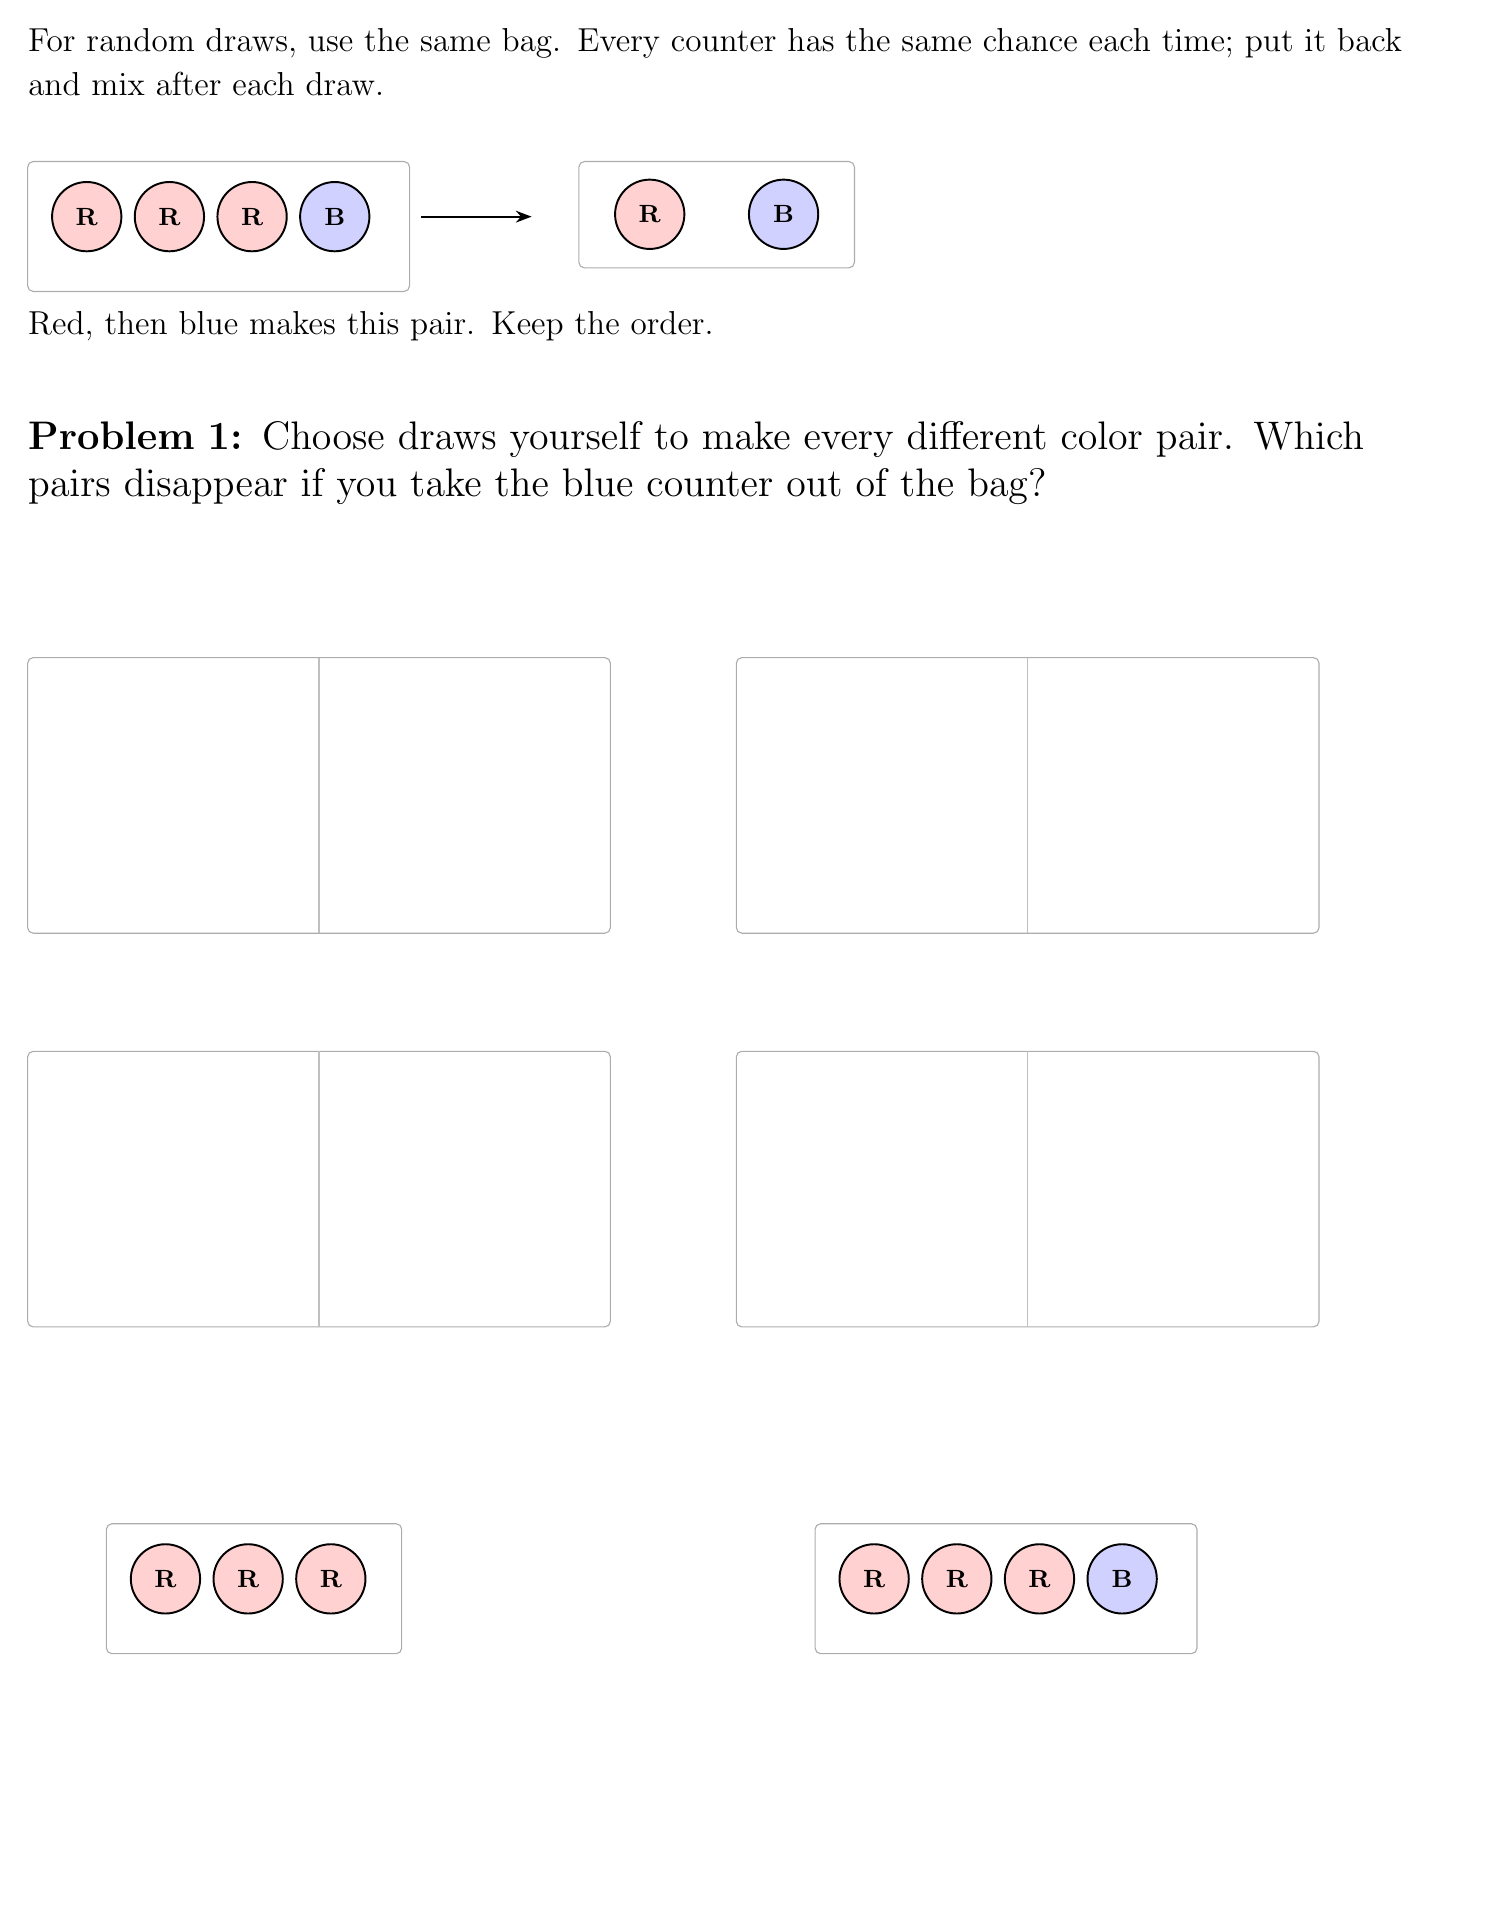
\begin{tikzpicture}[x=1cm,y=1cm]\path[use as bounding box] (0,0) rectangle (18.2,-23.6);
\node[anchor=north west,text width=18cm,inner sep=0pt,font=\fontsize{13}{16}\selectfont] at (0,0) {For random draws, use the same bag. Every counter has the same chance each time; put it back and mix after each draw.};
\draw[gray!65,rounded corners=2pt] (0,-1.7) rectangle (4.8500000000000005,-3.35);
\draw[fill=red!18,line width=.7pt] (0.75,-2.4) circle (0.44);
\node[font=\bfseries\small] at (0.75,-2.4) {R};
\draw[fill=red!18,line width=.7pt] (1.8,-2.4) circle (0.44);
\node[font=\bfseries\small] at (1.8,-2.4) {R};
\draw[fill=red!18,line width=.7pt] (2.85,-2.4) circle (0.44);
\node[font=\bfseries\small] at (2.85,-2.4) {R};
\draw[fill=blue!18,line width=.7pt] (3.9000000000000004,-2.4) circle (0.44);
\node[font=\bfseries\small] at (3.9000000000000004,-2.4) {B};
\draw[gray!65,rounded corners=2pt] (7,-1.7) rectangle (10.5,-3.05);
\draw[fill=red!18,line width=.7pt] (7.9,-2.37) circle (0.44);
\node[font=\bfseries\small] at (7.9,-2.37) {R};
\draw[fill=blue!18,line width=.7pt] (9.6,-2.37) circle (0.44);
\node[font=\bfseries\small] at (9.6,-2.37) {B};
\draw[-{Stealth[length=2mm]},line width=.8pt] (5,-2.4) -- (6.4,-2.4) node[midway,above,font=\small] {};
\node[anchor=north west,text width=18cm,inner sep=0pt,font=\fontsize{13}{16}\selectfont] at (0,-3.6) {Red, then blue makes this pair. Keep the order.};
\node[anchor=north west,text width=18cm,inner sep=0pt,font=\fontsize{14}{17}\selectfont] at (0,-5) {\textbf{Problem 1:} Choose draws yourself to make every different color pair. Which pairs disappear if you take the blue counter out of the bag?};
\draw[gray!65,rounded corners=2pt] (0,-8) rectangle (7.4,-11.5);
\draw[gray!50] (3.7,-8) -- (3.7,-11.5);
\draw[gray!65,rounded corners=2pt] (9,-8) rectangle (16.4,-11.5);
\draw[gray!50] (12.7,-8) -- (12.7,-11.5);
\draw[gray!65,rounded corners=2pt] (0,-13) rectangle (7.4,-16.5);
\draw[gray!50] (3.7,-13) -- (3.7,-16.5);
\draw[gray!65,rounded corners=2pt] (9,-13) rectangle (16.4,-16.5);
\draw[gray!50] (12.7,-13) -- (12.7,-16.5);
\draw[gray!65,rounded corners=2pt] (1,-19) rectangle (4.75,-20.65);
\draw[fill=red!18,line width=.7pt] (1.75,-19.7) circle (0.44);
\node[font=\bfseries\small] at (1.75,-19.7) {R};
\draw[fill=red!18,line width=.7pt] (2.8,-19.7) circle (0.44);
\node[font=\bfseries\small] at (2.8,-19.7) {R};
\draw[fill=red!18,line width=.7pt] (3.85,-19.7) circle (0.44);
\node[font=\bfseries\small] at (3.85,-19.7) {R};
\draw[gray!65,rounded corners=2pt] (10,-19) rectangle (14.850000000000001,-20.65);
\draw[fill=red!18,line width=.7pt] (10.75,-19.7) circle (0.44);
\node[font=\bfseries\small] at (10.75,-19.7) {R};
\draw[fill=red!18,line width=.7pt] (11.8,-19.7) circle (0.44);
\node[font=\bfseries\small] at (11.8,-19.7) {R};
\draw[fill=red!18,line width=.7pt] (12.85,-19.7) circle (0.44);
\node[font=\bfseries\small] at (12.85,-19.7) {R};
\draw[fill=blue!18,line width=.7pt] (13.9,-19.7) circle (0.44);
\node[font=\bfseries\small] at (13.9,-19.7) {B};
\end{tikzpicture}
\newpage
\noindent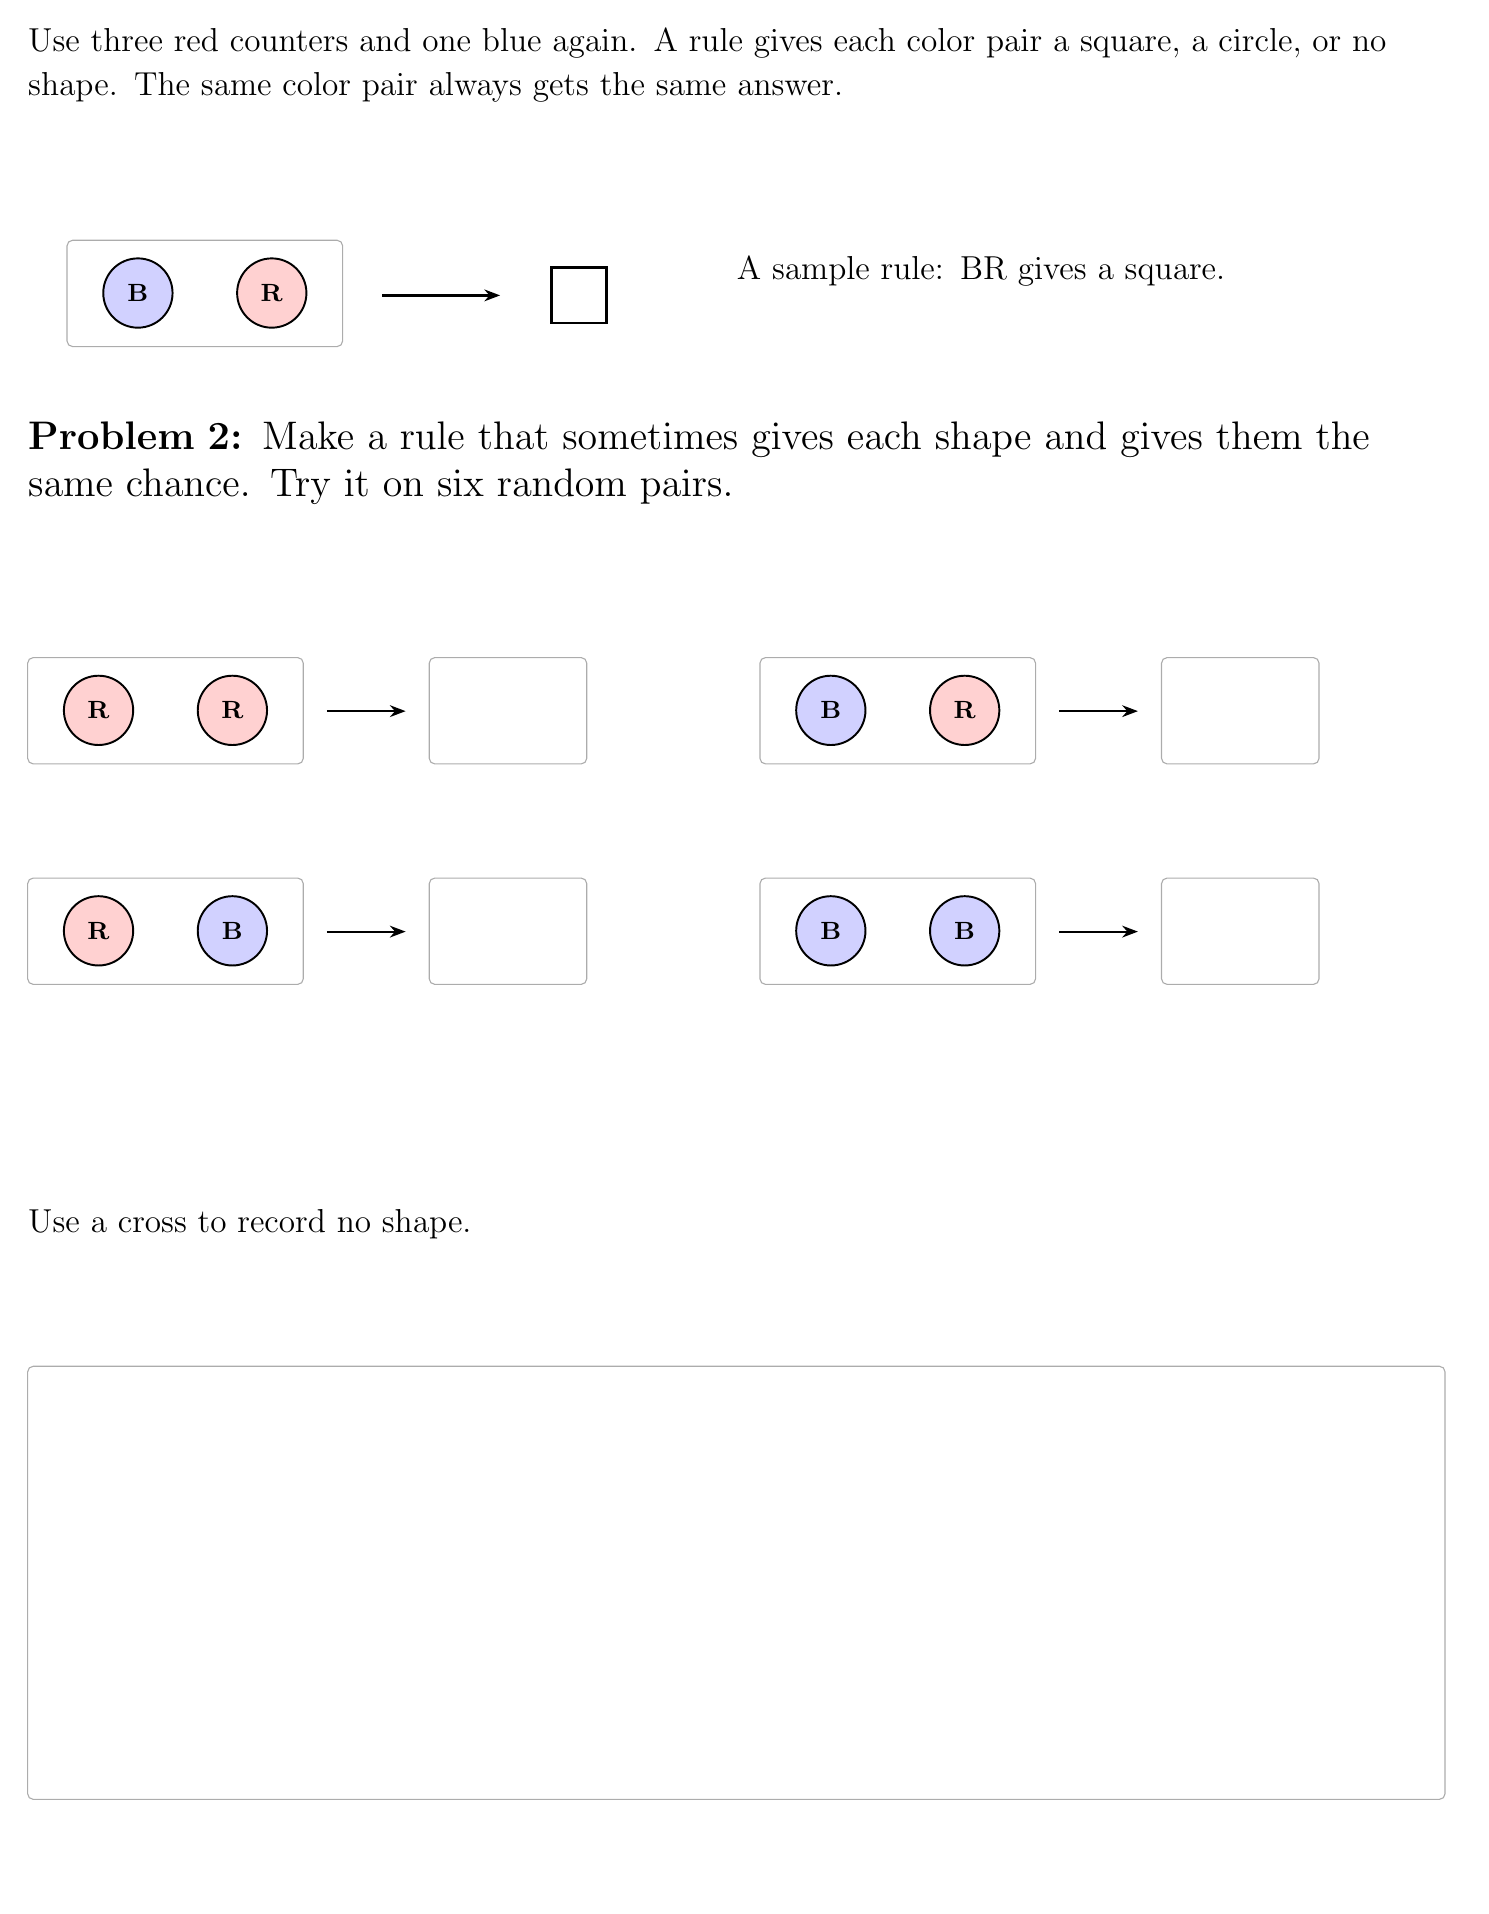
\begin{tikzpicture}[x=1cm,y=1cm]\path[use as bounding box] (0,0) rectangle (18.2,-23.6);
\node[anchor=north west,text width=18cm,inner sep=0pt,font=\fontsize{13}{16}\selectfont] at (0,0) {Use three red counters and one blue again. A rule gives each color pair a square, a circle, or no shape. The same color pair always gets the same answer.};
\draw[gray!65,rounded corners=2pt] (0.5,-2.7) rectangle (4.0,-4.050000000000001);
\draw[fill=blue!18,line width=.7pt] (1.4,-3.37) circle (0.44);
\node[font=\bfseries\small] at (1.4,-3.37) {B};
\draw[fill=red!18,line width=.7pt] (3.1,-3.37) circle (0.44);
\node[font=\bfseries\small] at (3.1,-3.37) {R};
\draw[-{Stealth[length=2mm]},line width=.8pt] (4.5,-3.4) -- (6,-3.4) node[midway,above,font=\small] {};
\draw[line width=1pt] (6.65,-3.75) rectangle (7.35,-3.05);
\node[anchor=north west,text width=8.5cm,inner sep=0pt,font=\fontsize{12}{15}\selectfont] at (9,-2.9) {A sample rule: BR gives a square.};
\node[anchor=north west,text width=18cm,inner sep=0pt,font=\fontsize{14}{17}\selectfont] at (0,-5) {\textbf{Problem 2:} Make a rule that sometimes gives each shape and gives them the same chance. Try it on six random pairs.};
\draw[gray!65,rounded corners=2pt] (0,-8.0) rectangle (3.5,-9.35);
\draw[fill=red!18,line width=.7pt] (0.9,-8.67) circle (0.44);
\node[font=\bfseries\small] at (0.9,-8.67) {R};
\draw[fill=red!18,line width=.7pt] (2.6,-8.67) circle (0.44);
\node[font=\bfseries\small] at (2.6,-8.67) {R};
\draw[-{Stealth[length=2mm]},line width=.8pt] (3.8,-8.68) -- (4.8,-8.68) node[midway,above,font=\small] {};
\draw[gray!65,rounded corners=2pt] (5.1,-8.0) rectangle (7.1,-9.35);
\draw[gray!65,rounded corners=2pt] (0,-10.8) rectangle (3.5,-12.15);
\draw[fill=red!18,line width=.7pt] (0.9,-11.47) circle (0.44);
\node[font=\bfseries\small] at (0.9,-11.47) {R};
\draw[fill=blue!18,line width=.7pt] (2.6,-11.47) circle (0.44);
\node[font=\bfseries\small] at (2.6,-11.47) {B};
\draw[-{Stealth[length=2mm]},line width=.8pt] (3.8,-11.48) -- (4.8,-11.48) node[midway,above,font=\small] {};
\draw[gray!65,rounded corners=2pt] (5.1,-10.8) rectangle (7.1,-12.15);
\draw[gray!65,rounded corners=2pt] (9.3,-8.0) rectangle (12.8,-9.35);
\draw[fill=blue!18,line width=.7pt] (10.200000000000001,-8.67) circle (0.44);
\node[font=\bfseries\small] at (10.200000000000001,-8.67) {B};
\draw[fill=red!18,line width=.7pt] (11.9,-8.67) circle (0.44);
\node[font=\bfseries\small] at (11.9,-8.67) {R};
\draw[-{Stealth[length=2mm]},line width=.8pt] (13.100000000000001,-8.68) -- (14.100000000000001,-8.68) node[midway,above,font=\small] {};
\draw[gray!65,rounded corners=2pt] (14.4,-8.0) rectangle (16.4,-9.35);
\draw[gray!65,rounded corners=2pt] (9.3,-10.8) rectangle (12.8,-12.15);
\draw[fill=blue!18,line width=.7pt] (10.200000000000001,-11.47) circle (0.44);
\node[font=\bfseries\small] at (10.200000000000001,-11.47) {B};
\draw[fill=blue!18,line width=.7pt] (11.9,-11.47) circle (0.44);
\node[font=\bfseries\small] at (11.9,-11.47) {B};
\draw[-{Stealth[length=2mm]},line width=.8pt] (13.100000000000001,-11.48) -- (14.100000000000001,-11.48) node[midway,above,font=\small] {};
\draw[gray!65,rounded corners=2pt] (14.4,-10.8) rectangle (16.4,-12.15);
\node[anchor=north west,text width=18cm,inner sep=0pt,font=\fontsize{13}{16}\selectfont] at (0,-15) {Use a cross to record no shape.};
\draw[gray!65,rounded corners=2pt] (0,-17) rectangle (18,-22.5);
\end{tikzpicture}
\newpage
\noindent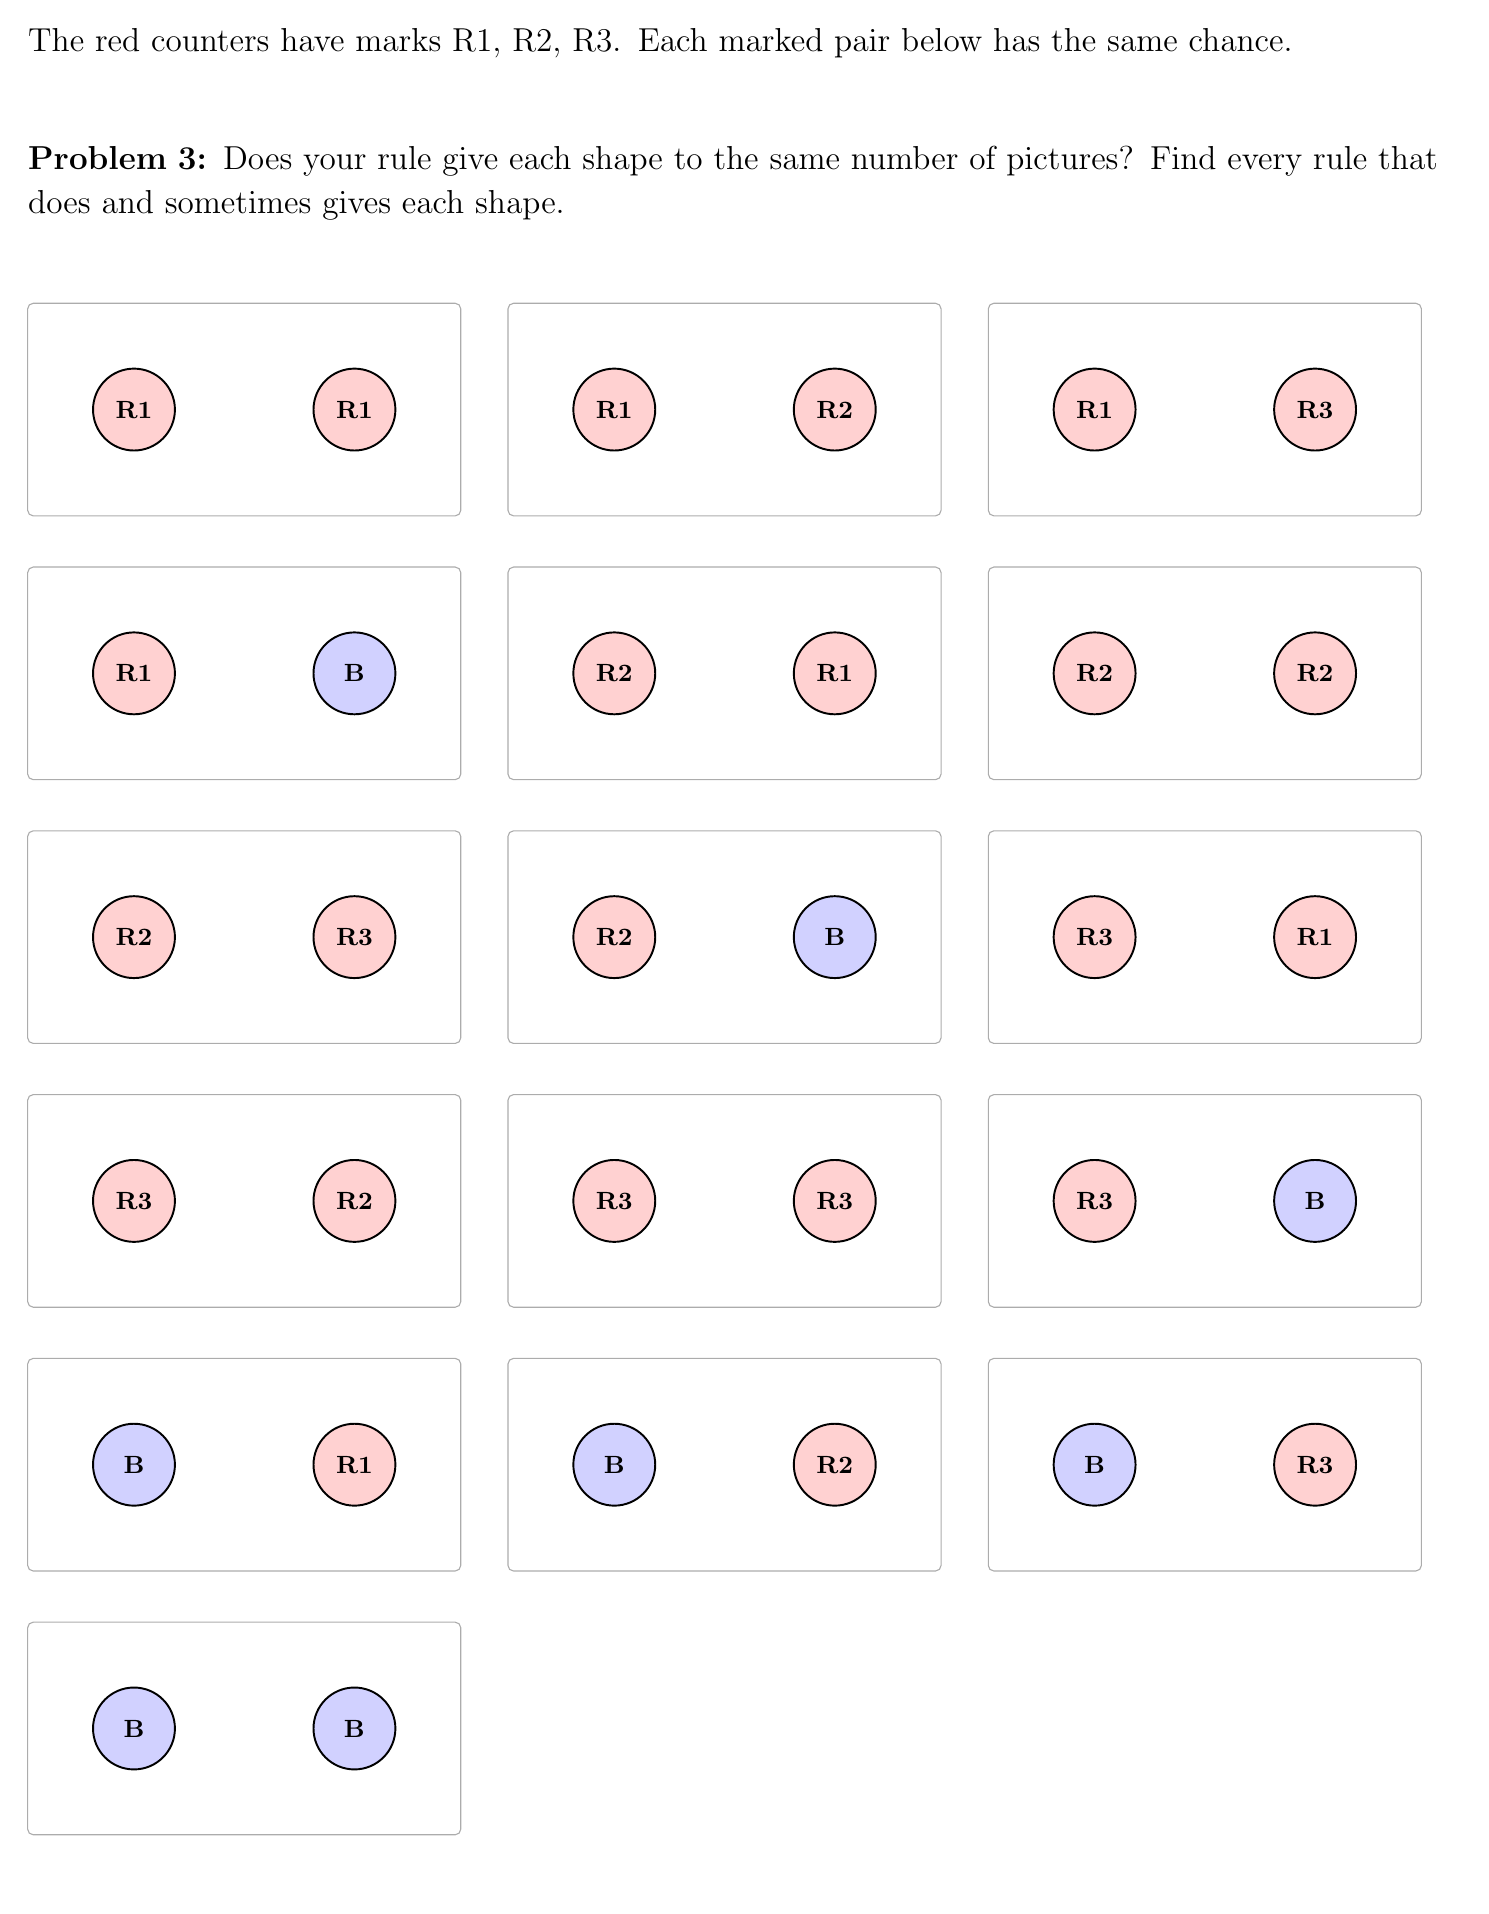
\begin{tikzpicture}[x=1cm,y=1cm]\path[use as bounding box] (0,0) rectangle (18.2,-23.6);
\node[anchor=north west,text width=18cm,inner sep=0pt,font=\fontsize{12}{15}\selectfont] at (0,0) {The red counters have marks R1, R2, R3. Each marked pair below has the same chance.};
\node[anchor=north west,text width=18cm,inner sep=0pt,font=\fontsize{13}{16}\selectfont] at (0,-1.5) {\textbf{Problem 3:} Does your rule give each shape to the same number of pictures? Find every rule that does and sometimes gives each shape.};
\draw[gray!65,rounded corners=2pt] (0.0,-3.5) rectangle (5.5,-6.2);
\draw[fill=red!18,line width=.7pt] (1.35,-4.85) circle (0.52);
\node[font=\bfseries\small] at (1.35,-4.85) {R1};
\draw[fill=red!18,line width=.7pt] (4.15,-4.85) circle (0.52);
\node[font=\bfseries\small] at (4.15,-4.85) {R1};
\draw[gray!65,rounded corners=2pt] (6.1,-3.5) rectangle (11.6,-6.2);
\draw[fill=red!18,line width=.7pt] (7.449999999999999,-4.85) circle (0.52);
\node[font=\bfseries\small] at (7.449999999999999,-4.85) {R1};
\draw[fill=red!18,line width=.7pt] (10.25,-4.85) circle (0.52);
\node[font=\bfseries\small] at (10.25,-4.85) {R2};
\draw[gray!65,rounded corners=2pt] (12.2,-3.5) rectangle (17.7,-6.2);
\draw[fill=red!18,line width=.7pt] (13.549999999999999,-4.85) circle (0.52);
\node[font=\bfseries\small] at (13.549999999999999,-4.85) {R1};
\draw[fill=red!18,line width=.7pt] (16.35,-4.85) circle (0.52);
\node[font=\bfseries\small] at (16.35,-4.85) {R3};
\draw[gray!65,rounded corners=2pt] (0.0,-6.85) rectangle (5.5,-9.55);
\draw[fill=red!18,line width=.7pt] (1.35,-8.2) circle (0.52);
\node[font=\bfseries\small] at (1.35,-8.2) {R1};
\draw[fill=blue!18,line width=.7pt] (4.15,-8.2) circle (0.52);
\node[font=\bfseries\small] at (4.15,-8.2) {B};
\draw[gray!65,rounded corners=2pt] (6.1,-6.85) rectangle (11.6,-9.55);
\draw[fill=red!18,line width=.7pt] (7.449999999999999,-8.2) circle (0.52);
\node[font=\bfseries\small] at (7.449999999999999,-8.2) {R2};
\draw[fill=red!18,line width=.7pt] (10.25,-8.2) circle (0.52);
\node[font=\bfseries\small] at (10.25,-8.2) {R1};
\draw[gray!65,rounded corners=2pt] (12.2,-6.85) rectangle (17.7,-9.55);
\draw[fill=red!18,line width=.7pt] (13.549999999999999,-8.2) circle (0.52);
\node[font=\bfseries\small] at (13.549999999999999,-8.2) {R2};
\draw[fill=red!18,line width=.7pt] (16.35,-8.2) circle (0.52);
\node[font=\bfseries\small] at (16.35,-8.2) {R2};
\draw[gray!65,rounded corners=2pt] (0.0,-10.2) rectangle (5.5,-12.899999999999999);
\draw[fill=red!18,line width=.7pt] (1.35,-11.549999999999999) circle (0.52);
\node[font=\bfseries\small] at (1.35,-11.549999999999999) {R2};
\draw[fill=red!18,line width=.7pt] (4.15,-11.549999999999999) circle (0.52);
\node[font=\bfseries\small] at (4.15,-11.549999999999999) {R3};
\draw[gray!65,rounded corners=2pt] (6.1,-10.2) rectangle (11.6,-12.899999999999999);
\draw[fill=red!18,line width=.7pt] (7.449999999999999,-11.549999999999999) circle (0.52);
\node[font=\bfseries\small] at (7.449999999999999,-11.549999999999999) {R2};
\draw[fill=blue!18,line width=.7pt] (10.25,-11.549999999999999) circle (0.52);
\node[font=\bfseries\small] at (10.25,-11.549999999999999) {B};
\draw[gray!65,rounded corners=2pt] (12.2,-10.2) rectangle (17.7,-12.899999999999999);
\draw[fill=red!18,line width=.7pt] (13.549999999999999,-11.549999999999999) circle (0.52);
\node[font=\bfseries\small] at (13.549999999999999,-11.549999999999999) {R3};
\draw[fill=red!18,line width=.7pt] (16.35,-11.549999999999999) circle (0.52);
\node[font=\bfseries\small] at (16.35,-11.549999999999999) {R1};
\draw[gray!65,rounded corners=2pt] (0.0,-13.55) rectangle (5.5,-16.25);
\draw[fill=red!18,line width=.7pt] (1.35,-14.9) circle (0.52);
\node[font=\bfseries\small] at (1.35,-14.9) {R3};
\draw[fill=red!18,line width=.7pt] (4.15,-14.9) circle (0.52);
\node[font=\bfseries\small] at (4.15,-14.9) {R2};
\draw[gray!65,rounded corners=2pt] (6.1,-13.55) rectangle (11.6,-16.25);
\draw[fill=red!18,line width=.7pt] (7.449999999999999,-14.9) circle (0.52);
\node[font=\bfseries\small] at (7.449999999999999,-14.9) {R3};
\draw[fill=red!18,line width=.7pt] (10.25,-14.9) circle (0.52);
\node[font=\bfseries\small] at (10.25,-14.9) {R3};
\draw[gray!65,rounded corners=2pt] (12.2,-13.55) rectangle (17.7,-16.25);
\draw[fill=red!18,line width=.7pt] (13.549999999999999,-14.9) circle (0.52);
\node[font=\bfseries\small] at (13.549999999999999,-14.9) {R3};
\draw[fill=blue!18,line width=.7pt] (16.35,-14.9) circle (0.52);
\node[font=\bfseries\small] at (16.35,-14.9) {B};
\draw[gray!65,rounded corners=2pt] (0.0,-16.9) rectangle (5.5,-19.599999999999998);
\draw[fill=blue!18,line width=.7pt] (1.35,-18.25) circle (0.52);
\node[font=\bfseries\small] at (1.35,-18.25) {B};
\draw[fill=red!18,line width=.7pt] (4.15,-18.25) circle (0.52);
\node[font=\bfseries\small] at (4.15,-18.25) {R1};
\draw[gray!65,rounded corners=2pt] (6.1,-16.9) rectangle (11.6,-19.599999999999998);
\draw[fill=blue!18,line width=.7pt] (7.449999999999999,-18.25) circle (0.52);
\node[font=\bfseries\small] at (7.449999999999999,-18.25) {B};
\draw[fill=red!18,line width=.7pt] (10.25,-18.25) circle (0.52);
\node[font=\bfseries\small] at (10.25,-18.25) {R2};
\draw[gray!65,rounded corners=2pt] (12.2,-16.9) rectangle (17.7,-19.599999999999998);
\draw[fill=blue!18,line width=.7pt] (13.549999999999999,-18.25) circle (0.52);
\node[font=\bfseries\small] at (13.549999999999999,-18.25) {B};
\draw[fill=red!18,line width=.7pt] (16.35,-18.25) circle (0.52);
\node[font=\bfseries\small] at (16.35,-18.25) {R3};
\draw[gray!65,rounded corners=2pt] (0.0,-20.25) rectangle (5.5,-22.95);
\draw[fill=blue!18,line width=.7pt] (1.35,-21.6) circle (0.52);
\node[font=\bfseries\small] at (1.35,-21.6) {B};
\draw[fill=blue!18,line width=.7pt] (4.15,-21.6) circle (0.52);
\node[font=\bfseries\small] at (4.15,-21.6) {B};
\end{tikzpicture}
\newpage
\noindent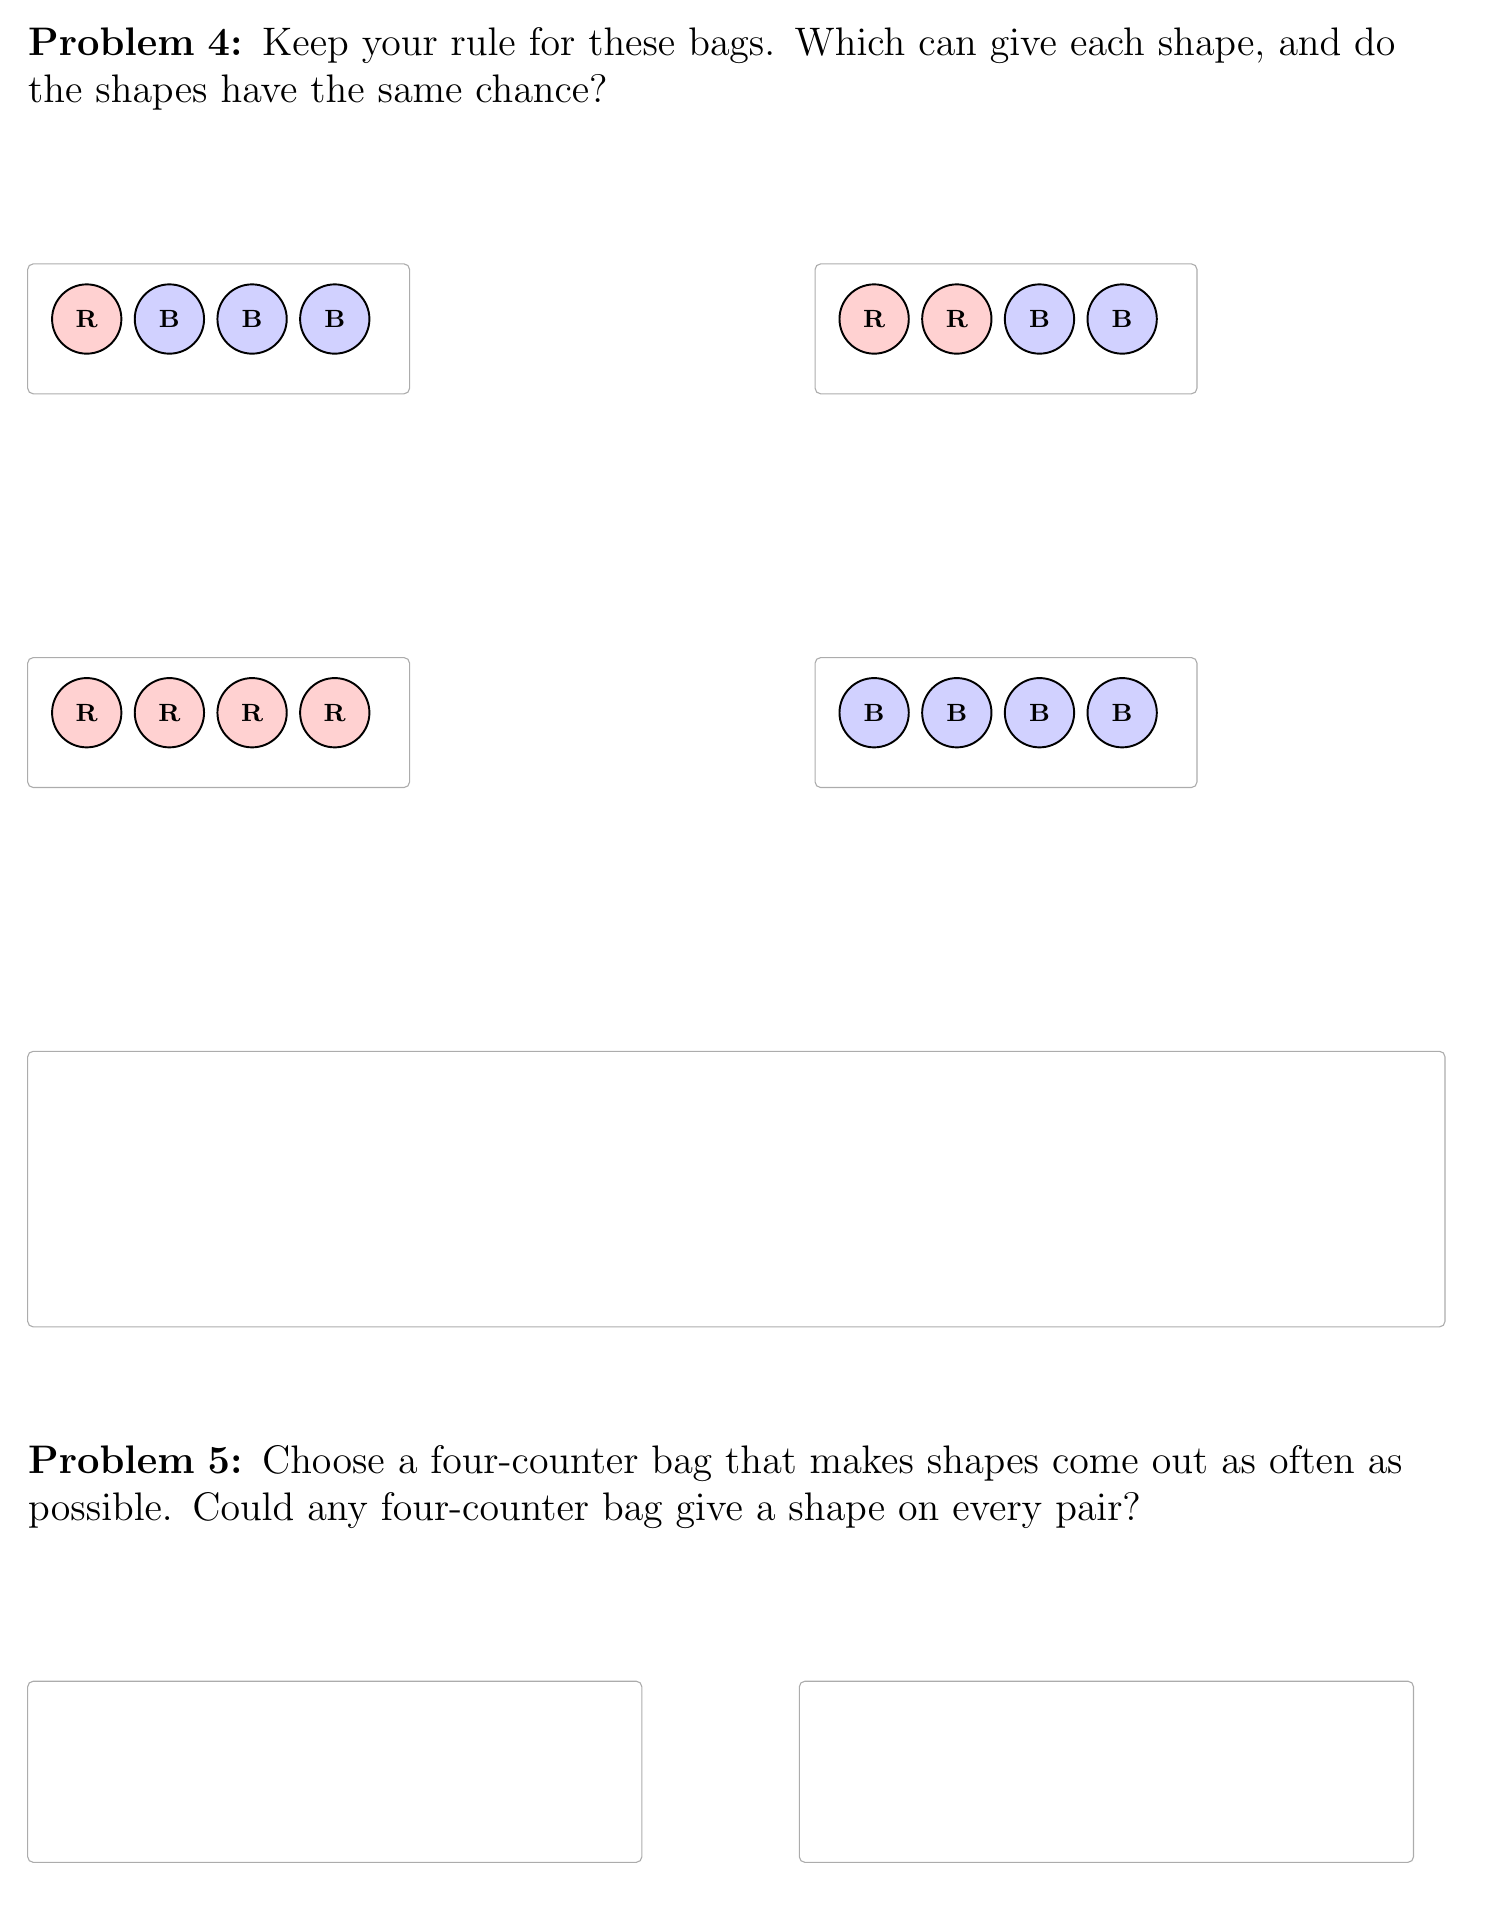
\begin{tikzpicture}[x=1cm,y=1cm]\path[use as bounding box] (0,0) rectangle (18.2,-23.6);
\node[anchor=north west,text width=18cm,inner sep=0pt,font=\fontsize{14}{17}\selectfont] at (0,0) {\textbf{Problem 4:} Keep your rule for these bags. Which can give each shape, and do the shapes have the same chance?};
\draw[gray!65,rounded corners=2pt] (0,-3) rectangle (4.8500000000000005,-4.65);
\draw[fill=red!18,line width=.7pt] (0.75,-3.7) circle (0.44);
\node[font=\bfseries\small] at (0.75,-3.7) {R};
\draw[fill=blue!18,line width=.7pt] (1.8,-3.7) circle (0.44);
\node[font=\bfseries\small] at (1.8,-3.7) {B};
\draw[fill=blue!18,line width=.7pt] (2.85,-3.7) circle (0.44);
\node[font=\bfseries\small] at (2.85,-3.7) {B};
\draw[fill=blue!18,line width=.7pt] (3.9000000000000004,-3.7) circle (0.44);
\node[font=\bfseries\small] at (3.9000000000000004,-3.7) {B};
\draw[gray!65,rounded corners=2pt] (10,-3) rectangle (14.850000000000001,-4.65);
\draw[fill=red!18,line width=.7pt] (10.75,-3.7) circle (0.44);
\node[font=\bfseries\small] at (10.75,-3.7) {R};
\draw[fill=red!18,line width=.7pt] (11.8,-3.7) circle (0.44);
\node[font=\bfseries\small] at (11.8,-3.7) {R};
\draw[fill=blue!18,line width=.7pt] (12.85,-3.7) circle (0.44);
\node[font=\bfseries\small] at (12.85,-3.7) {B};
\draw[fill=blue!18,line width=.7pt] (13.9,-3.7) circle (0.44);
\node[font=\bfseries\small] at (13.9,-3.7) {B};
\draw[gray!65,rounded corners=2pt] (0,-8) rectangle (4.8500000000000005,-9.65);
\draw[fill=red!18,line width=.7pt] (0.75,-8.7) circle (0.44);
\node[font=\bfseries\small] at (0.75,-8.7) {R};
\draw[fill=red!18,line width=.7pt] (1.8,-8.7) circle (0.44);
\node[font=\bfseries\small] at (1.8,-8.7) {R};
\draw[fill=red!18,line width=.7pt] (2.85,-8.7) circle (0.44);
\node[font=\bfseries\small] at (2.85,-8.7) {R};
\draw[fill=red!18,line width=.7pt] (3.9000000000000004,-8.7) circle (0.44);
\node[font=\bfseries\small] at (3.9000000000000004,-8.7) {R};
\draw[gray!65,rounded corners=2pt] (10,-8) rectangle (14.850000000000001,-9.65);
\draw[fill=blue!18,line width=.7pt] (10.75,-8.7) circle (0.44);
\node[font=\bfseries\small] at (10.75,-8.7) {B};
\draw[fill=blue!18,line width=.7pt] (11.8,-8.7) circle (0.44);
\node[font=\bfseries\small] at (11.8,-8.7) {B};
\draw[fill=blue!18,line width=.7pt] (12.85,-8.7) circle (0.44);
\node[font=\bfseries\small] at (12.85,-8.7) {B};
\draw[fill=blue!18,line width=.7pt] (13.9,-8.7) circle (0.44);
\node[font=\bfseries\small] at (13.9,-8.7) {B};
\draw[gray!65,rounded corners=2pt] (0,-13) rectangle (18,-16.5);
\node[anchor=north west,text width=18cm,inner sep=0pt,font=\fontsize{14}{17}\selectfont] at (0,-18) {\textbf{Problem 5:} Choose a four-counter bag that makes shapes come out as often as possible. Could any four-counter bag give a shape on every pair?};
\draw[gray!65,rounded corners=2pt] (0,-21) rectangle (7.8,-23.3);
\draw[gray!65,rounded corners=2pt] (9.8,-21) rectangle (17.6,-23.3);
\end{tikzpicture}
\newpage
\noindent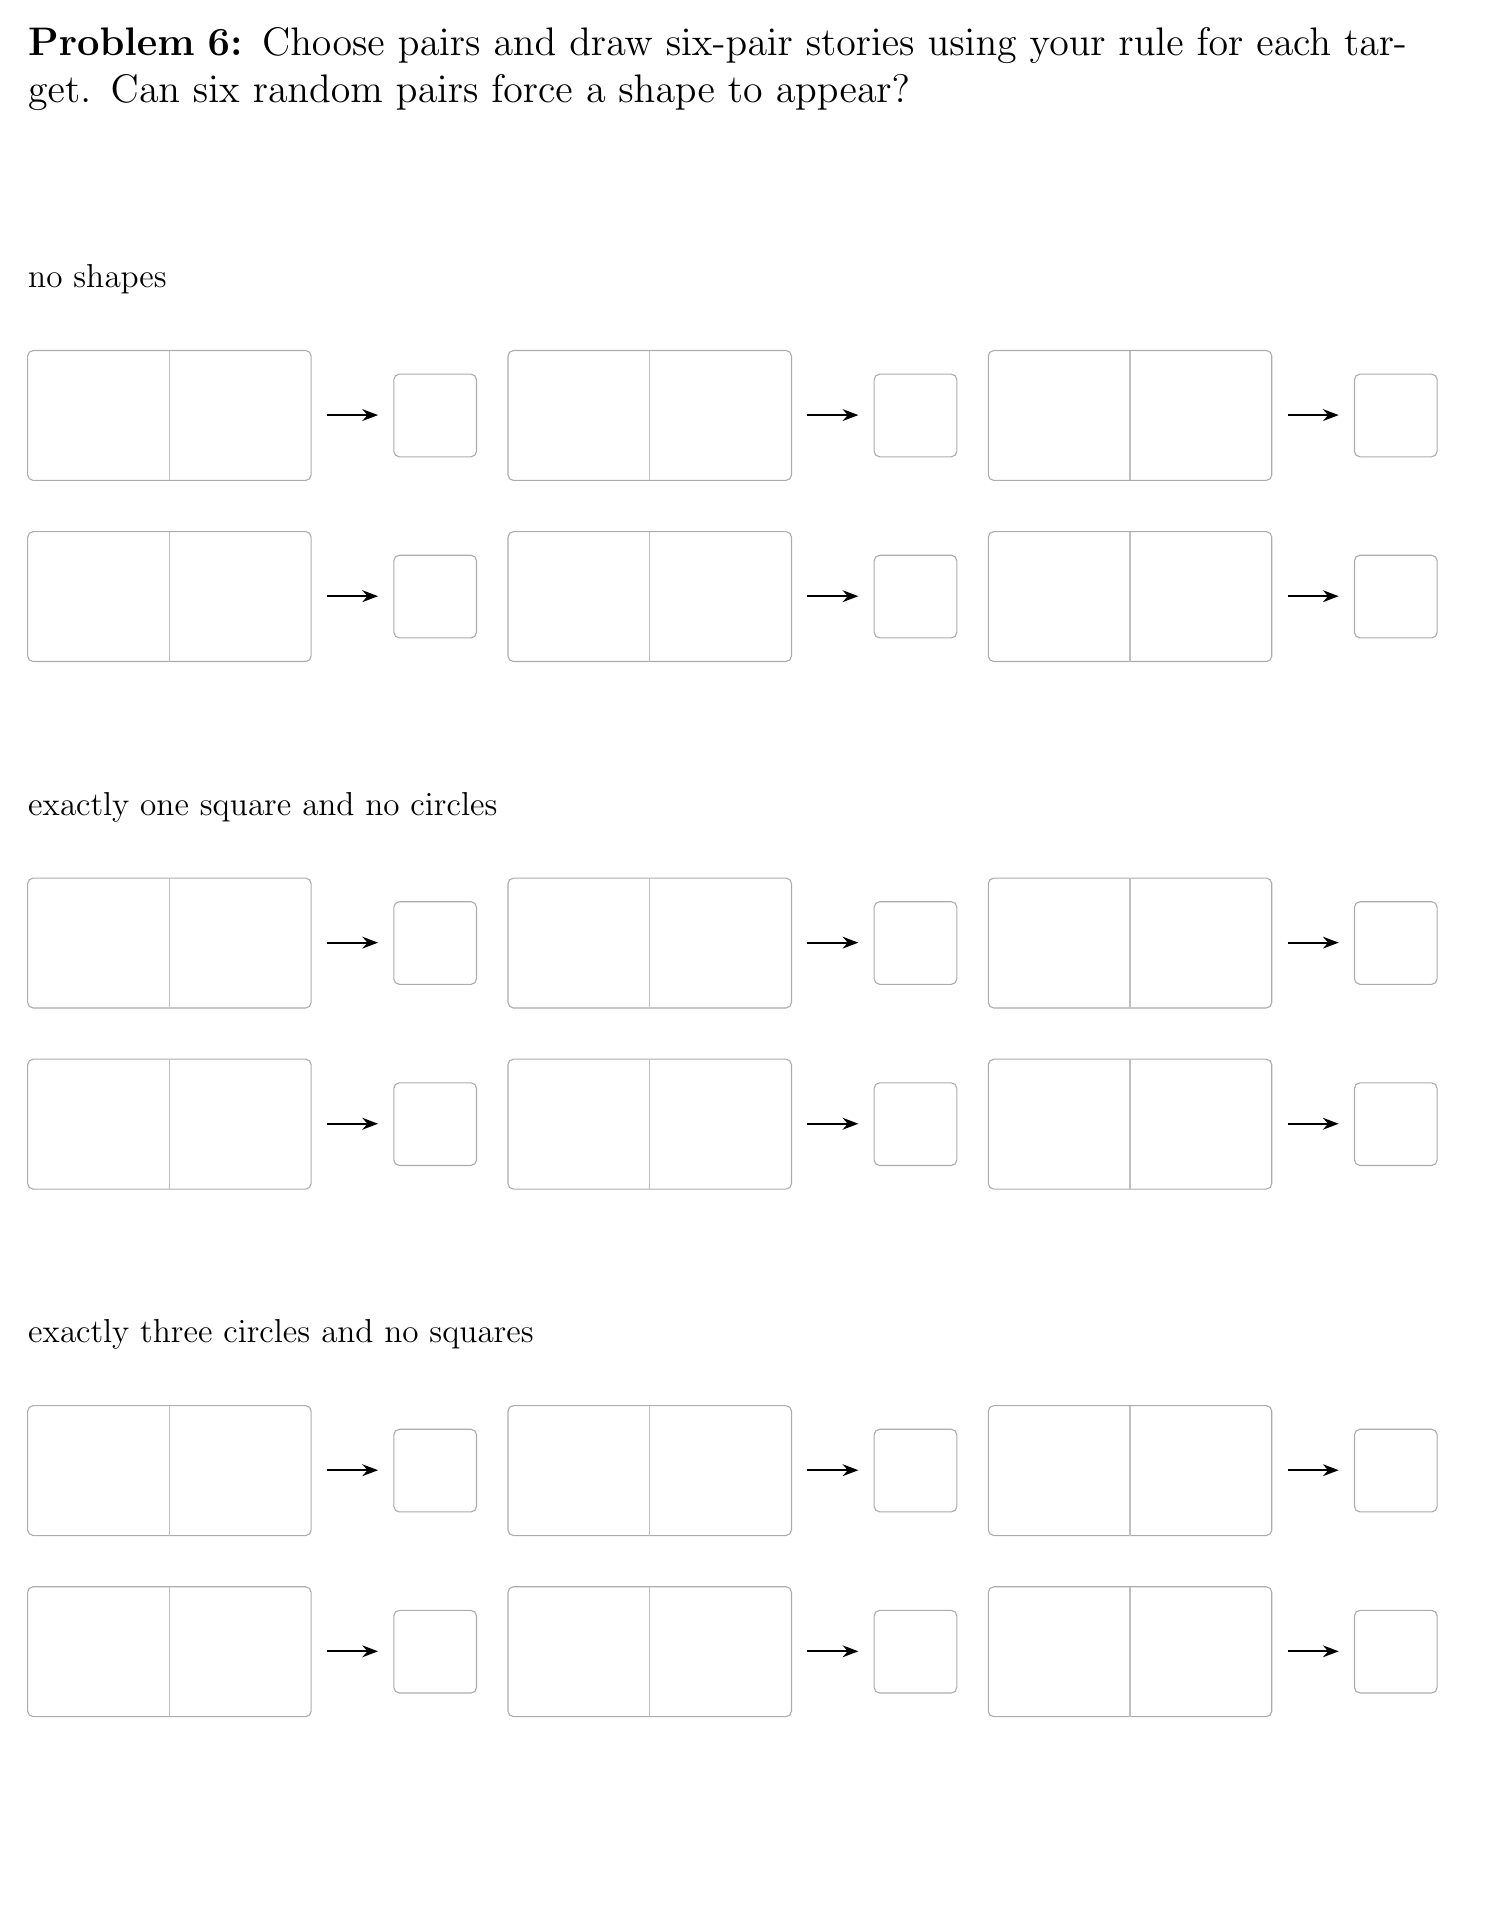
\begin{tikzpicture}[x=1cm,y=1cm]\path[use as bounding box] (0,0) rectangle (18.2,-23.6);
\node[anchor=north west,text width=18cm,inner sep=0pt,font=\fontsize{14}{17}\selectfont] at (0,0) {\textbf{Problem 6:} Choose pairs and draw six-pair stories using your rule for each target. Can six random pairs force a shape to appear?};
\node[anchor=north west,text width=18cm,inner sep=0pt,font=\fontsize{13}{16}\selectfont] at (0,-3) {no shapes};
\draw[gray!65,rounded corners=2pt] (0.0,-4.1) rectangle (3.6,-5.75);
\draw[gray!50] (1.8,-4.1) -- (1.8,-5.75);
\draw[-{Stealth[length=2mm]},line width=.8pt] (3.8,-4.92) -- (4.45,-4.92) node[midway,above,font=\small] {};
\draw[gray!65,rounded corners=2pt] (4.65,-4.3999999999999995) rectangle (5.7,-5.449999999999999);
\draw[gray!65,rounded corners=2pt] (6.1,-4.1) rectangle (9.7,-5.75);
\draw[gray!50] (7.8999999999999995,-4.1) -- (7.8999999999999995,-5.75);
\draw[-{Stealth[length=2mm]},line width=.8pt] (9.899999999999999,-4.92) -- (10.55,-4.92) node[midway,above,font=\small] {};
\draw[gray!65,rounded corners=2pt] (10.75,-4.3999999999999995) rectangle (11.8,-5.449999999999999);
\draw[gray!65,rounded corners=2pt] (12.2,-4.1) rectangle (15.799999999999999,-5.75);
\draw[gray!50] (14.0,-4.1) -- (14.0,-5.75);
\draw[-{Stealth[length=2mm]},line width=.8pt] (16.0,-4.92) -- (16.65,-4.92) node[midway,above,font=\small] {};
\draw[gray!65,rounded corners=2pt] (16.85,-4.3999999999999995) rectangle (17.900000000000002,-5.449999999999999);
\draw[gray!65,rounded corners=2pt] (0.0,-6.3999999999999995) rectangle (3.6,-8.049999999999999);
\draw[gray!50] (1.8,-6.3999999999999995) -- (1.8,-8.049999999999999);
\draw[-{Stealth[length=2mm]},line width=.8pt] (3.8,-7.22) -- (4.45,-7.22) node[midway,above,font=\small] {};
\draw[gray!65,rounded corners=2pt] (4.65,-6.699999999999999) rectangle (5.7,-7.749999999999999);
\draw[gray!65,rounded corners=2pt] (6.1,-6.3999999999999995) rectangle (9.7,-8.049999999999999);
\draw[gray!50] (7.8999999999999995,-6.3999999999999995) -- (7.8999999999999995,-8.049999999999999);
\draw[-{Stealth[length=2mm]},line width=.8pt] (9.899999999999999,-7.22) -- (10.55,-7.22) node[midway,above,font=\small] {};
\draw[gray!65,rounded corners=2pt] (10.75,-6.699999999999999) rectangle (11.8,-7.749999999999999);
\draw[gray!65,rounded corners=2pt] (12.2,-6.3999999999999995) rectangle (15.799999999999999,-8.049999999999999);
\draw[gray!50] (14.0,-6.3999999999999995) -- (14.0,-8.049999999999999);
\draw[-{Stealth[length=2mm]},line width=.8pt] (16.0,-7.22) -- (16.65,-7.22) node[midway,above,font=\small] {};
\draw[gray!65,rounded corners=2pt] (16.85,-6.699999999999999) rectangle (17.900000000000002,-7.749999999999999);
\node[anchor=north west,text width=18cm,inner sep=0pt,font=\fontsize{13}{16}\selectfont] at (0,-9.7) {exactly one square and no circles};
\draw[gray!65,rounded corners=2pt] (0.0,-10.799999999999999) rectangle (3.6,-12.45);
\draw[gray!50] (1.8,-10.799999999999999) -- (1.8,-12.45);
\draw[-{Stealth[length=2mm]},line width=.8pt] (3.8,-11.62) -- (4.45,-11.62) node[midway,above,font=\small] {};
\draw[gray!65,rounded corners=2pt] (4.65,-11.1) rectangle (5.7,-12.15);
\draw[gray!65,rounded corners=2pt] (6.1,-10.799999999999999) rectangle (9.7,-12.45);
\draw[gray!50] (7.8999999999999995,-10.799999999999999) -- (7.8999999999999995,-12.45);
\draw[-{Stealth[length=2mm]},line width=.8pt] (9.899999999999999,-11.62) -- (10.55,-11.62) node[midway,above,font=\small] {};
\draw[gray!65,rounded corners=2pt] (10.75,-11.1) rectangle (11.8,-12.15);
\draw[gray!65,rounded corners=2pt] (12.2,-10.799999999999999) rectangle (15.799999999999999,-12.45);
\draw[gray!50] (14.0,-10.799999999999999) -- (14.0,-12.45);
\draw[-{Stealth[length=2mm]},line width=.8pt] (16.0,-11.62) -- (16.65,-11.62) node[midway,above,font=\small] {};
\draw[gray!65,rounded corners=2pt] (16.85,-11.1) rectangle (17.900000000000002,-12.15);
\draw[gray!65,rounded corners=2pt] (0.0,-13.099999999999998) rectangle (3.6,-14.749999999999998);
\draw[gray!50] (1.8,-13.099999999999998) -- (1.8,-14.749999999999998);
\draw[-{Stealth[length=2mm]},line width=.8pt] (3.8,-13.919999999999998) -- (4.45,-13.919999999999998) node[midway,above,font=\small] {};
\draw[gray!65,rounded corners=2pt] (4.65,-13.399999999999999) rectangle (5.7,-14.45);
\draw[gray!65,rounded corners=2pt] (6.1,-13.099999999999998) rectangle (9.7,-14.749999999999998);
\draw[gray!50] (7.8999999999999995,-13.099999999999998) -- (7.8999999999999995,-14.749999999999998);
\draw[-{Stealth[length=2mm]},line width=.8pt] (9.899999999999999,-13.919999999999998) -- (10.55,-13.919999999999998) node[midway,above,font=\small] {};
\draw[gray!65,rounded corners=2pt] (10.75,-13.399999999999999) rectangle (11.8,-14.45);
\draw[gray!65,rounded corners=2pt] (12.2,-13.099999999999998) rectangle (15.799999999999999,-14.749999999999998);
\draw[gray!50] (14.0,-13.099999999999998) -- (14.0,-14.749999999999998);
\draw[-{Stealth[length=2mm]},line width=.8pt] (16.0,-13.919999999999998) -- (16.65,-13.919999999999998) node[midway,above,font=\small] {};
\draw[gray!65,rounded corners=2pt] (16.85,-13.399999999999999) rectangle (17.900000000000002,-14.45);
\node[anchor=north west,text width=18cm,inner sep=0pt,font=\fontsize{13}{16}\selectfont] at (0,-16.4) {exactly three circles and no squares};
\draw[gray!65,rounded corners=2pt] (0.0,-17.5) rectangle (3.6,-19.15);
\draw[gray!50] (1.8,-17.5) -- (1.8,-19.15);
\draw[-{Stealth[length=2mm]},line width=.8pt] (3.8,-18.32) -- (4.45,-18.32) node[midway,above,font=\small] {};
\draw[gray!65,rounded corners=2pt] (4.65,-17.8) rectangle (5.7,-18.85);
\draw[gray!65,rounded corners=2pt] (6.1,-17.5) rectangle (9.7,-19.15);
\draw[gray!50] (7.8999999999999995,-17.5) -- (7.8999999999999995,-19.15);
\draw[-{Stealth[length=2mm]},line width=.8pt] (9.899999999999999,-18.32) -- (10.55,-18.32) node[midway,above,font=\small] {};
\draw[gray!65,rounded corners=2pt] (10.75,-17.8) rectangle (11.8,-18.85);
\draw[gray!65,rounded corners=2pt] (12.2,-17.5) rectangle (15.799999999999999,-19.15);
\draw[gray!50] (14.0,-17.5) -- (14.0,-19.15);
\draw[-{Stealth[length=2mm]},line width=.8pt] (16.0,-18.32) -- (16.65,-18.32) node[midway,above,font=\small] {};
\draw[gray!65,rounded corners=2pt] (16.85,-17.8) rectangle (17.900000000000002,-18.85);
\draw[gray!65,rounded corners=2pt] (0.0,-19.8) rectangle (3.6,-21.45);
\draw[gray!50] (1.8,-19.8) -- (1.8,-21.45);
\draw[-{Stealth[length=2mm]},line width=.8pt] (3.8,-20.62) -- (4.45,-20.62) node[midway,above,font=\small] {};
\draw[gray!65,rounded corners=2pt] (4.65,-20.1) rectangle (5.7,-21.150000000000002);
\draw[gray!65,rounded corners=2pt] (6.1,-19.8) rectangle (9.7,-21.45);
\draw[gray!50] (7.8999999999999995,-19.8) -- (7.8999999999999995,-21.45);
\draw[-{Stealth[length=2mm]},line width=.8pt] (9.899999999999999,-20.62) -- (10.55,-20.62) node[midway,above,font=\small] {};
\draw[gray!65,rounded corners=2pt] (10.75,-20.1) rectangle (11.8,-21.150000000000002);
\draw[gray!65,rounded corners=2pt] (12.2,-19.8) rectangle (15.799999999999999,-21.45);
\draw[gray!50] (14.0,-19.8) -- (14.0,-21.45);
\draw[-{Stealth[length=2mm]},line width=.8pt] (16.0,-20.62) -- (16.65,-20.62) node[midway,above,font=\small] {};
\draw[gray!65,rounded corners=2pt] (16.85,-20.1) rectangle (17.900000000000002,-21.150000000000002);
\end{tikzpicture}
\end{document}
